\documentclass[a4paper, 10pt]{article}
\usepackage{helvet}
\renewcommand{\familydefault}{\sfdefault}
\usepackage{pgf}
\usepackage{eurosym}
\usepackage{graphicx}
\usepackage{wasysym}
\usepackage{hyperref}
\usepackage{listings}
\usepackage{pxfonts}
\usepackage{verbatim}
\usepackage{color}
\usepackage{xcolor}
\usepackage{wrapfig}
\usepackage{enumitem}
\usepackage{booktabs}
\usepackage{gensymb}
\usepackage{tabularx}
\usepackage{currfile}

\hypersetup{
    bookmarks=true,         % show bookmarks bar?
    unicode=true,          % non-Latin characters in Acrobat’s bookmarks
    pdftoolbar=true,        % show Acrobat’s toolbar?
    pdfmenubar=true,        % show Acrobat’s menu?
    pdffitwindow=true,     % window fit to page when opened
    pdftitle={Assessments},    % title
    pdfauthor={Paul Vesey},     % author
    pdfsubject={Building Information Modelling },   % subject of the document
    pdfcreator={},   % creator of the document
    pdfproducer={xelatex}, % producer of the document
    pdfkeywords={'Graphics' }, % list of keywords
    pdfnewwindow=true,      % links in new PDF window
    colorlinks=true,       % false: boxed links; true: colored links
    linkcolor=violet,          % color of internal links (change box color with linkbordercolor)
    citecolor=magenta,        % color of links to bibliography
    filecolor=red,      % color of file links
    urlcolor=blue           % color of external links
}

\setlength\parindent{0pt}
\begin{document}

\lstset{language=HTML,
				basicstyle=\small,
				breaklines=true,
        numbers=left,
        numberstyle=\tiny,
        showstringspaces=false,
        aboveskip=-20pt,
        frame=leftline
        }
				
\begin{figure}
	\centering
	
\includegraphics[width=0.5\linewidth]{./Assignments/img/LITlogo}
\end{figure}


\begin{tabularx}{\textwidth}{ |l|X| }
	\hline
	\textbf{Subject:} & Revit MEP\\
	\textbf{Course:} & Building Information Modelling with Revit MEP\\
	\textbf{Session:} & Autumn 2021\\
	\textbf{Lecturer:} & Paul Vesey \footnotesize{BEng, MIE, HDip}\\
	\textbf{Filename:} & \currfilebase\\
	\hline
\end{tabularx}



\vspace{0.25cm}	
	

\part*{Assignment 3 (33\%) - Miscellaneous Activities in 3 Parts}



\begin{tabularx}{\textwidth}{ |X|X| }
	\hline
	\textbf{Issue Date:} & As stated on MS Teams \\
	\hline 
	\textbf{Submission Date:}  & As stated on MS Teams  \\
	\hline
\end{tabularx}



\section*{Assignment Outline}



In these exercises you are required to create a number of new items and modify the existing designs created during Assignment 2 and Assignment 3.  This assignment consists of 3 parts, each of which has its own set of deliverables and submission file(s).

\newpage
\section*{Part 1 - Domestic Building Details}



\begin{figure}
	\centering
	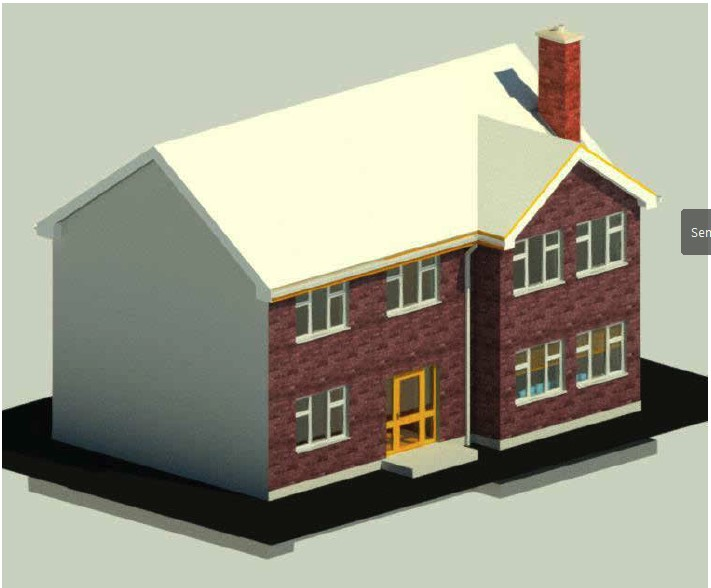
\includegraphics[width=1.0\linewidth]{img/House}
	\caption{Domestic Building - Indicative only}
	\label{fig:house}
\end{figure}



Using the Residential model developed for Assignment 1, make the following amendments to your design.
\begin{enumerate}
	\item\label{itm:roof} Roof: Change the roof name to Domestic Roof with Conc Tile finish, and change the roof make-up to 
	\begin{itemize}
		\item 30mm Concrete roofing tile on,
		\item 38mm (Wood Lumber) Battens on,
		\item 2mm Roofing Felt on,
		\item 166mm Truss
	\end{itemize}
	\item\label{itm:FirstFloor} First Floor: Add 12mm Oak Flooring layer on top of the suspended timber floor make-up
	\item\label{itm:GroundFloor} Ground Floor: Edit and Duplicate the ground floor type and rename as 'Ground Floor - Domestic w Oakwood Finish'.  Edit the construction to reflect the following build-up:
	\begin{itemize}
		\item 6mm Oakwood Flooring finish on,
		\item 80mm Sand \& Cement Screed on,
		\item 100mm Rigid Insulation on,
		\item 150mm In-situ Concrete on,
		\item LDPE DPM / Radon Membrane on,
		\item 50mm Sand on,
		\item 200mm Site Hardcore
	\end{itemize}
	\item Produce the following 3D View and 3 Call-out views. Place these views on a new sheet, A105.  Include annotations and dimensions as necessary.
	\begin{itemize}
		\item Call-out Detail of the Roof / External Wall interface @ 1:20
		\item Call-out Detail of the First Floor / External Wall interface @ 1:20
		\item Call-out Detail of the Ground Floor / External Wall / Foundation interface @ 1:20
	\end{itemize}
	\item The filenames should be of the form used in PAS/BS 1192.  In this case, it will \textit{RARC03-\#\#\#-00-ZZ-M3-A-301-A1-P01}, where \#\#\# is replaced by the last 3 digits of your K-number. An example would be \textbf{'RARC03-920-00-ZZ-M3-A-3001-A1-P01'}, for K-number K20001920.
\end{enumerate}
Make use of the Masking and Component tools, and the 'Repeating Detail' functionality in Revit.  Annotations should include, at a minimum, the construction information outlined in items \ref{itm:roof}, \ref{itm:FirstFloor} and \ref{itm:GroundFloor}. 






\newpage

\section*{Part 2 - Commercial Building Details}

\begin{figure}
	\centering
	\includegraphics[width=1.0\linewidth]{img/RetailBuilding}
	\caption{Commercial Building}
	\label{fig:retailbuilding}
\end{figure}



Using the Commercial Building model developed for Assignment 2, make the following amendments to your design. 

\begin{enumerate}
	\item Roof: Create a curved extruded roof similar to the diagram shown in Figure \ref{fig:retailbuilding}
	
	\item 3D Views: Create 3 Autodesk 360 rendered images and import them into a new sheet, A-207.
	\begin{itemize}
		\item External view of the building looking through the curtain wall glazing
		\item Internal view of one retail unit facing the curtain wall, and picking up the stairs
		\item Internal view of your choice from the First Floor landing 
	\end{itemize} 
	\item Solar Study: Create a solar study for the 16\textsuperscript{th} of June 2018 and place a view of 14:30 hours onto sheet A-207.  Render your image using the 'shaded' setting; do not fully render.  
	\item Walk-throughs: Create the following walk-throughs using the 'Shaded' setting.  Do not fully render the animation.  The maximum number of frames required is 300.
	\item Sloping Toposurface: Create a sloped topographical surface (approx 80m x 90m) incorporating a slope from approx 5m hight at the rear, and 8.0m out from the building, to -225mm at the front of the building, and over the front area of the site.
	\begin{itemize}
		\item Create a Building Pad incorporating an 8.0m hard-stand area to the rear and sides of the Retail Unit block and approx 15.0m at the front
		\item Create a parking area for cars to the front of the building
		\item Provide an access road from the edge of the Site to the car park.
		\item Add street lighting, trees, and other components from the 'Entourage', 'Site' and 'Planting' libraries as necessary 
	\end{itemize}
	\item The filenames should be of the form used in PAS/BS 1192.  In this case, it will \textit{RARC03-\#\#\#-00-ZZ-M3-A-302-A1-P01}, where \#\#\# is replaced by the last 3 digits of your K-number. An example would be \textbf{'RARC03-920-00-ZZ-M3-A-302-A1-P01'}, for K-number K20001920.
\end{enumerate}

\newpage

\section*{Part 3 - Interoperability (File Exchange formats)}

Using your Assignment 1 Building, create or export the following file types from Revit
\begin{enumerate}
	\item Export the floor plan in Autocad .dwg format
	\item Export the default 3D view in FBX format.  FBX is used for many 3D applications as a semi-neutral format.  You do not need to set LOD or Boundary Edges.
	\item Export the floor plans in .gbXML format, used in Energy Analysis
	\item Make a .pdf of the floor plan
\end{enumerate}
The filenames should be of the form used in PAS/BS 1192.  In this case, it will \textit{RARC03-\#\#\#-00-ZZ-\$\$-A-001-A1-P01}, where \#\#\# is replaced by the last 3 digits of your K-number and \$\$ is the PAS codes for Drawings and Models. An example would be \textbf{'RARC03-920-00-ZZ-MR-A-001-A1-P01'}, for K-number K20001920, energy analysis model.  Please do not use spaces in the filename.\\ The codes are as follows: \\

\begin{tabularx}{\textwidth}{ |c|X| }
	\hline
	\textbf{Code} & \textbf{Usage} \\
	\hline 
	AF  & Animation File  \\
	CM  & Combined Model  \\
	CR  & Specific for Clash Detection  \\
	DR  & 2D Drawing  \\
	M2  & 2D Model  \\
	M3  & 3D Model  \\
	MR  & Model file for other renditions  \\
	VS  & Visualisation  \\
	\hline
\end{tabularx}


\end{document}